
%(BEGIN_QUESTION)
% Copyright 2013, Tony R. Kuphaldt, released under the Creative Commons Attribution License (v 1.0)
% This means you may do almost anything with this work of mine, so long as you give me proper credit

Examine this process trend showing the PV, SP, and Output of a loop controller:

$$\includegraphics[width=15.5cm]{i02635x01.eps}$$

Based on what you see here, determine the following:

\begin{itemize}
\item{} Whether this is an open-loop or a closed-loop response
\item{} Whether the controller is (or needs to be) {\it direct-acting} or {\it reverse-acting}
\item{} If possible, identify any problems with the field instrumentation
\item{} If possible, identify any problems with the controller PID tuning
\item{} Qualitatively identify the kind of PID tuning we will need for robust control
\end{itemize}

\underbar{file i02635}
%(END_QUESTION)





%(BEGIN_ANSWER)

This is a {\it closed-loop test}, based on the fact the output signal responds dynamically to the changing process variable, as well as to the step-change in setpoint.

\vskip 10pt

This is a {\it reverse-acting} controller: the output steps up when the setpoint steps up (implying the output would step down if the process variable stepped up).

\vskip 10pt

There do not appear to be any field instrumentation problems revealed in this trend.  A manual-mode (open-loop) test would be more informative in that regard, and it appears as though the process possesses a multiple-order lag, but the time scale of this lag seems modest.  It might not be a bad idea to look around for sources of lag time (e.g. thermowell mass, improperly inserted temperature probe), just to see if the response time might be improved a bit.  Another possibility explaining the lag time would be a transmitter (or controller input block) configured with too much filtering (damping), adding a single-order lag to whatever lag(s) the process itself already possesses.

\vskip 10pt
  
The controller tuning is clearly inappropriate for this process, and should be much more aggressive than it is right now.  Note how the PV is taking a long time to reach the new SP, and how the controller output is ramping down at a very leisurely pace.

\vskip 10pt

This process appears to be self-regulating, and so we know we must have some integral action in the controller.  The existence of multiple-order lag makes this loop a good candidate for moderate derivative action.

%(END_ANSWER)





%(BEGIN_NOTES)


%INDEX% Process troubleshooting: diagnosing problem via trend recording

%(END_NOTES)


